\section{分布族与参数}
\label{sec:dfam-families}

回到章首那枚三面骰子。它的概率规律就是一张表$(p_0,p_1,p_2)$，三个数非负、和为$1$。在知道更多之前，这样的表都有可能；知道平均点数是$1$以后，只剩一部分表还有资格。这里有两件不同的事：一件是哪些概率规律被允许，另一件是怎样给被允许的规律编号。本节先讨论前者，再讨论后者，并说明编号时可能出现的重复。

\subsection{候选分布的范围}
\label{sec:dfam-candidates}

设$(\mathcal{X},\mathcal{F}_{\mathcal{X}})$是取值空间，记$\mathcal{P}(\mathcal{X})$为其上全体概率测度。研究一个随机现象时，我们往往不能断定它的分布是哪一个，只能根据机制和已知事实圈出一个范围。

\begin{definition}[分布族]
\label{def:dfam-family}
$\mathcal{P}(\mathcal{X})$的任一非空子集$\mathcal{C}$称为$\mathcal{X}$上的一个\term{分布族}（family of distributions）。
\end{definition}

分布族的成员是概率测度本身，不是随机变量，也不是参数。说“$X$的分布属于$\mathcal{C}$”，是在对$X$的概率规律提出要求，而不是在对$X$的取值或某个数字提出要求。下面先在有限取值空间上看这些要求长什么样。

\paragraph{有限概率表的三角形}
取$\mathcal{X}=\{0,1,2\}$。一个概率测度由三个数$p_x=P(\{x\})$确定，全体概率测度对应集合
\begin{equation}
  \Delta_2=\{(p_0,p_1,p_2):p_x\geq0,\ p_0+p_1+p_2=1\}.
  \label{eq:dfam-simplex}
\end{equation}
它是$\mathbb{R}^{3}$中以三个坐标向量为顶点的三角形，即第~\ref{chap:multivariate-distributions}章的标准单纯形。顶点是集中在一点的分布，三条边是恰有一个结果概率为零的分布，内部是三个结果都可能出现的分布。图~\ref{fig:dfam-simplex-candidates}把这个三角形摊平画出。

候选范围的第一类要求是固定支持。要求三个结果都有正概率，候选集合是三角形的内部；已知结果$2$不会出现，候选集合是$p_2=0$那条边。这类要求只看哪些点上有质量，不看质量有多少。

第二类要求是矩约束。要求$\mathbb{E}_P[X]=1$，就是
\[
  p_1+2p_2=1 .
\]
与$p_0+p_1+p_2=1$相减，得到
\[
  p_0=p_2 .
\]
所以满足约束的表形如$(t,1-2t,t)$，$0\leq t\leq1/2$，这是从顶点$(0,1,0)$到底边中点$(1/2,0,1/2)$的一条线段。均匀表$(1/3,1/3,1/3)$在线段上，点$(1/2,0,1/2)$也在线段上，它把一半质量放在$0$、一半放在$2$，平均同样是$1$。

\begin{BookInlineFigure}
  \centering
  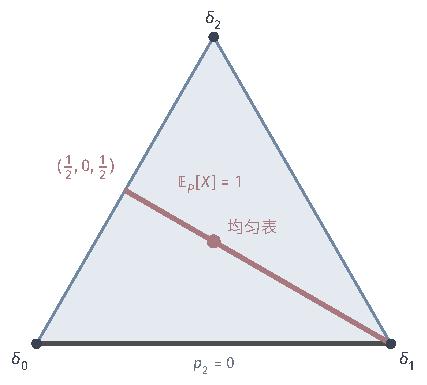
\includegraphics[width=72.4mm]{figures/07-probability/04-distribution-analysis/tikz/dfam-simplex-candidates/figure.pdf}
  \caption{$\{0,1,2\}$上的全体概率表构成三角形$\Delta_2$，三个顶点是点质量$\delta_0,\delta_1,\delta_2$。浅蓝区域是三个结果都有正概率的内部；深灰粗边$p_2=0$是不出现结果$2$的表，也是相对计数测度$\nu$（支撑$\{0,1\}$）绝对连续的表；红色线段是满足$\mathbb{E}_P[X]=1$的表$(t,1-2t,t)$，红点为均匀表。}
  \label{fig:dfam-simplex-candidates}
\end{BookInlineFigure}

第三类要求是相对某个\term{参考测度}（reference measure）$\nu$绝对连续，即凡$\nu(B)=0$的集合都有$P(B)=0$。在$\{0,1,2\}$上取$\nu$为$\{0,1\}$上的计数测度，$\nu(\{2\})=0$，于是$P\ll\nu$恰好意味着$p_2=0$，与固定支持的要求相同。在有限空间上两者没有差别；在连续空间上，绝对连续才保证密度$\mathrm{d}P/\mathrm{d}\nu$存在（Radon–Nikodym定理，见\BookChapterRef{chap:measure-densities}{卷四第8章“测度的密度”}），它是用密度描述分布族的前提。

几类要求可以叠加。同时要求三个结果都可能出现、平均为$1$，候选集合就是去掉两个端点的开线段。每加一条要求，三角形里剩下的部分就小一些，但它仍然是概率表的集合，我们还没有给其中的表起任何名字。

\paragraph{给定均值的密度}
换到连续情形，差别就显出来了。设读数取值于$(0,\infty)$，要求分布相对Lebesgue测度绝对连续且均值为$1$，候选集合是
\begin{equation}
  \mathcal{C}_1=\Bigl\{f\geq0:\int_0^\infty f(x)\,\mathrm{d}x=1,\ \int_0^\infty xf(x)\,\mathrm{d}x=1\Bigr\}.
  \label{eq:dfam-mean-one}
\end{equation}
这里两个密度若几乎处处相等，就看作同一个分布。$\operatorname{Exp}(1)$的密度$\mathrm{e}^{-x}$、$\operatorname{Gamma}(2,2)$的密度$4x\mathrm{e}^{-2x}$和$\operatorname{Unif}(0,2)$的密度$1/2$（$0<x<2$）都在$\mathcal{C}_1$里，形状却各不相同，见图~\ref{fig:dfam-mean-one-densities}。点质量$\delta_1$的均值也是$1$，但它不相对Lebesgue测度绝对连续，被第一个要求排除在外。

\begin{BookInlineFigure}
  \centering
  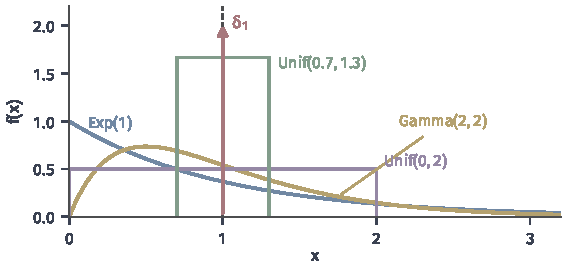
\includegraphics[width=96mm]{figures/07-probability/04-distribution-analysis/matplotlib/dfam-mean-one-densities/figure.pdf}
  \caption{均值都等于$1$的几个分布。蓝线为$\operatorname{Exp}(1)$，黄线为$\operatorname{Gamma}(2,2)$，紫线为$\operatorname{Unif}(0,2)$，绿线为$(1-a,1+a)$上的均匀密度（$a=0.3$）；红色箭头表示点质量$\delta_1$，它没有相对Lebesgue测度的密度。深灰竖线标出均值$x=1$。}
  \label{fig:dfam-mean-one-densities}
\end{BookInlineFigure}

$\mathcal{C}_1$大到什么程度？取$0<a_1<a_2<\cdots<a_n<1$，令$g_k$为区间$(1-a_k,1+a_k)$上的均匀密度。区间关于$1$对称，所以每个$g_k$的均值都是$1$。对任意权重$c_k\geq0$、$\sum_kc_k=1$，凸组合$\sum_kc_kg_k$仍非负、积分为$1$、均值为$1$，所以它也在$\mathcal{C}_1$中。

这$n$个密度线性无关。设$\sum_kc_kg_k=0$几乎处处成立。在区间$(1+a_{n-1},1+a_n)$上只有$g_n$不为零，所以$c_n=0$；去掉$g_n$后对$g_{n-1}$重复同样的论证，依次得到所有$c_k=0$。由于$n$可以任意大，$\mathcal{C}_1$不包含在任何有限维仿射子空间中，因而不能写成有限个固定密度带参数的线性组合。

这说明候选范围与参数表示是两回事。三角形上的线段可以用一个数$t$编号，$\mathcal{C}_1$却不能用有限个系数作线性编号。描述候选集合时不应预设它总有一个有限维参数；有限维的参数族是从候选集合中再挑出的一部分，挑法正是本章后面几节的内容。

\subsection{参数表示与可辨识性}
\label{sec:dfam-identifiability}

给分布编号，就是指定一个集合$\Theta$和一个映射$\bm{\theta}\mapsto P_{\bm{\theta}}$，让每个参数值对应一个概率测度。

\begin{definition}[参数化分布族]
\label{def:dfam-parametric-family}
设$\Theta$是一个集合，对每个$\bm{\theta}\in\Theta$给定$P_{\bm{\theta}}\in\mathcal{P}(\mathcal{X})$。分布族$\{P_{\bm{\theta}}:\bm{\theta}\in\Theta\}$称为以$\Theta$为\term{参数空间}（parameter space）的参数化分布族。若各$P_{\bm{\theta}}$都相对同一个参考测度$\nu$绝对连续，记其密度为$p_{\bm{\theta}}$。
\end{definition}

分布族是映射的像，参数化是映射本身。同一个族可以有许多参数化。Bernoulli族$\{\operatorname{Bern}(p):0<p<1\}$可以直接用$p$编号，也可以用$\eta\in\mathbb{R}$编号：
\[
  p=\frac{\mathrm{e}^{\eta}}{1+\mathrm{e}^{\eta}} .
\]
两种编号得到的分布集合完全相同，对应单纯形$\Delta_1$（一条线段）去掉两个端点，差别只在刻度：$p$在$(0,1)$上均匀刻度，$\eta$把靠近$0$和$1$的部分拉长到整条实轴。

\paragraph{重复的参数}
编号可能是冗余的。令$(a,b)\in(0,\infty)^2$对应$\operatorname{Bern}\bigl(a/(a+b)\bigr)$。$(1,2)$与$(2,4)$给出同一个分布$\operatorname{Bern}(1/3)$；更一般地，从原点出发的每条射线$\{(ca,cb):c>0\}$整条对应同一个分布，如图~\ref{fig:dfam-redundant-parameters}。两个参数，却只描述一个自由度的分布。

\begin{BookInlineFigure}
  \centering
  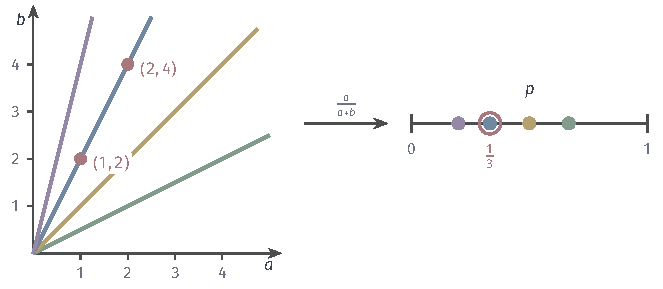
\includegraphics[width=112mm]{figures/07-probability/04-distribution-analysis/tikz/dfam-redundant-parameters/figure.pdf}
  \caption{冗余参数化$(a,b)\mapsto\operatorname{Bern}(a/(a+b))$。左：参数平面中，同一条射线上的点（同色）对应同一个分布，红点$(1,2)$与$(2,4)$都给出$\operatorname{Bern}(1/3)$。右：分布只由$p=a/(a+b)$决定，射线被压成线段$(0,1)$上的一点。}
  \label{fig:dfam-redundant-parameters}
\end{BookInlineFigure}

\begin{definition}[可辨识性]
\label{def:dfam-identifiable}
若对$\bm{\theta},\bm{\theta}'\in\Theta$，由$P_{\bm{\theta}}=P_{\bm{\theta}'}$总能推出$\bm{\theta}=\bm{\theta}'$，则称参数化$\bm{\theta}\mapsto P_{\bm{\theta}}$是\term{可辨识}（identifiable）的。
\end{definition}

可辨识就是参数到分布的映射是单射。这里的“分布相等”指两个概率测度在每个可测集上相等；用密度描述时，指$p_{\bm{\theta}}=p_{\bm{\theta}'}$相对$\nu$几乎处处成立。$\operatorname{Unif}[0,\theta]$与$\operatorname{Unif}(0,\theta)$的密度只在两个端点不同，它们是同一个分布，改动零测集上的值不产生新的参数。

可辨识性是参数化的性质，不是分布族的性质。上面的$(a,b)$参数化不可辨识，同一个Bernoulli族用$p$编号却可辨识。另一个常见的冗余来自参数只以组合形式出现：$(\theta_1,\theta_2)\mapsto\mathcal{N}(\theta_1+\theta_2,1)$中，直线$\theta_1+\theta_2=c$上的所有参数都给出$\mathcal{N}(c,1)$，分布只看得见和，看不见两个加数各是多少。

\paragraph{标签置换}
第~\ref{chap:random-vectors}章的混合分布带来另一种冗余。把两个高斯成分按权重相加，参数是$(w,\mu_1,\mu_2)$：
\[
  P_{(w,\mu_1,\mu_2)}=w\,\mathcal{N}(\mu_1,1)+(1-w)\,\mathcal{N}(\mu_2,1).
\]
交换两个成分的名字，得到
\[
  P_{(0.3,-1,2)}=P_{(0.7,2,-1)} .
\]
两组参数不同，分布却相同，这称为\term{标签置换}（label switching）。图~\ref{fig:dfam-label-switching}在$w=1/2$时画出$(\mu_1,\mu_2)$平面：关于对角线对称的两点给出同一个分布。

\begin{BookInlineFigure}
  \centering
  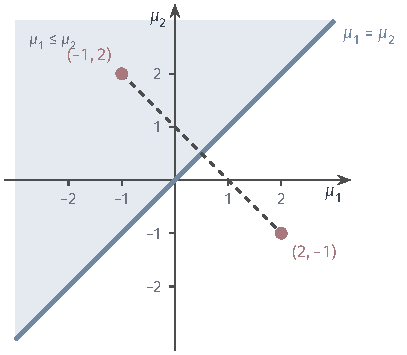
\includegraphics[width=68.9mm]{figures/07-probability/04-distribution-analysis/tikz/dfam-label-switching/figure.pdf}
  \caption{等权两成分高斯混合$\frac12\mathcal{N}(\mu_1,1)+\frac12\mathcal{N}(\mu_2,1)$的参数平面。关于对角线$\mu_1=\mu_2$对称的两点（红点$(-1,2)$与$(2,-1)$）给出同一个分布。限制在浅蓝的半平面$\mu_1\leq\mu_2$中，每个分布只剩一个参数。}
  \label{fig:dfam-label-switching}
\end{BookInlineFigure}

消除这种冗余有两个办法。一是缩小参数空间，例如只保留$\mu_1\leq\mu_2$的参数；二是承认参数只能确定到某种等价，把互相置换的参数看作同一个。两种办法都不改变分布族，只改变编号方式。混合表示中还有更多冗余，第~\ref{sec:dfam-mixture-nonuniqueness}节专门处理。

\paragraph{可辨识与能否从样本分辨}
可辨识性只问两个参数是否给出不同的分布，不问这种差别有多大。$\operatorname{Bern}(0.50)$与$\operatorname{Bern}(0.51)$是两个不同的分布，$p$参数化可辨识；可是各抛$100$次，正面次数的均值分别是$50$与$51$，标准差都约为$5$，两组次数的波动远大于均值之差，看一次试验结果几乎无法判断是哪一个。

另一个例子是$\theta\mapsto\mathcal{N}(\theta^{3},1)$。$\theta\mapsto\theta^{3}$是单射，所以它可辨识；但$\theta=0.1$与$\theta=0$对应的均值只差$0.001$，参数在$0$附近的变化几乎不改变分布。可辨识是分布层面的唯一性，是能否从数据推断参数的前提，但不是充分条件；有限样本下能多准确地估计参数，属于统计推断的问题，见\BookChapterRef{chap:parametric-statistical-inference}{卷八第1章“参数化统计推断”}。
